\documentclass{article}
\title{Social Movements, Science, Bureaucracy, and Democracy:\\ How mass participation shapes technocratic policymaking}

\author{DRAFT DISSERTATION RESEARCH PROPOSAL: \\ \\Devin Judge-Lord\\ Any thoughts on this project would be greatly appreciated: \href{mailto:JudgeLord@Wisc.edu}{JudgeLord@Wisc.edu}}
\date{\today} 

\usepackage{natbib}
  \bibpunct[: ]{(}{)}{;}{a}{}{,}

\usepackage[margin=.85in]{geometry} % margins % ipad geometry is 4X3
\usepackage{setspace} % line spacing
\usepackage{graphicx} % input graphics
%  \graphicspath{{./../output/graphics/}} % global path to graphics folder
\usepackage{float} % float parameters
\usepackage{placeins} % \FloatBarrier: prevent floats spilling across sections
\usepackage{subcaption} % subfloats with individual captions
\usepackage{multirow} % multicolumn and multirow
\usepackage{booktabs} %? for toprule, midrule etc
\usepackage{dcolumn} % decimal-aligned columns
\usepackage{hyperref} % hyperlinks
   \hypersetup{
     colorlinks = true, 
     citecolor = black, 
     linkcolor = blue,
     urlcolor = blue}
\usepackage{comment} % provides {comment} environment
\usepackage{enumitem} % allows [nosep] option for lists

\usepackage{tikz}
\def\checkmark{\tikz\fill[scale=0.4](0,.35) -- (.25,0) -- (1,.7) -- (.25,.15) -- cycle;} 
\usepackage{fancybox}


\begin{document}

\maketitle
% \texttt{NOTES FOR EPW: Thank you so much for your comments. This is a very early stage idea. I hope to pilot the design by working with one organization to run one campaign this spring. The study as proposed is extremely ambitious, potentially infeasible. As such, comments on three areas would be especially helpful: (1) modifications to make it more feasible, (2) outcome measures that are likely to see the strongest signal, and, relatedly (3) survey questions for organizational participants (see appendix). Getting the survey right for the pilot is most urgent.}

\abstract{
%This dissertation will examine the role of mass mobilization in agency policymaking. 
We lack systematic evidence on how civic actions such as protests, petitions, and large numbers of public comments on draft regulations shape the political environment in which agencies make policy. While some speculate that mass mobilization matters, the studies that come closest to addressing this question find no such evidence. Theories of bureaucratic policymaking seem to point in both directions and specific theories in either direction are lacking. Furthermore, the normative appeal of institutions like notice-and-comment rulemaking, rooted in ideas of direct democracy, depends on who participates, who is influential, and why---empirical questions that require a study on whether---and if so, why---mass participation matters. I aim to provide this study.

The first part assembles a theoretical foundation for understanding agency rulemaking as a political phenomenon that is occasionally a site of contentious debate and civic mobilization. I draw on scholarship in political science, law, and public administration and data on hundreds of thousands of rules made in the past 40 years.

The second part aims to identify mechanisms, both direct and indirect, by which mass mobilization may shape an agency's decisionmaking environment. I assess indirect mechanisms by measuring variation in external attention to rulemaking processes, especially by media and elected officials, and direct mechanisms by measuring the attention and meanings that agency staff give to public comments. For example, I examine the text of congressional, White House, inter-agency communications, and court opinions related to rulemaking processes as well as the text of proposed rules, public comments, agencies' responses to comments, and final rules. My aim is to identify any differences in the politics of rulemaking when large numbers of people participate from when they do not and whether these differences, if any, are associated with different policy outcomes.

The third part develops new methods to study the causal effects of mass mobilization through experimental manipulation of advocacy strategies and text analysis. This involves partnering with organizations to randomly assign strategies and surveying participating organizations before and after a mass-comment campaign to compare expert priors with outcomes. Public comment campaigns are not the only way to signal to agencies that large numbers of people are paying attention, but it is one signal that cannot be missed. It may also shape media attention and public discourse. Tracing the effects of campaign decisions on agencies' political environments will thus contribute to our understanding of the roles of advocacy organizations and the people they engage in policymaking.} %In this design, the number and text of public comments are the treatment and the text of bureaucrats' discussion of public comments and changes in policy are the response. 
\pagebreak
%\tableofcontents
%\onehalfspace
%\section{Context} 
%With the rise of the administrative state, bureaucratic policymaking has become a major site of policymaking and political contestation. In the years or decades between legislative enactments, federal agencies make legally-binding rules interpreting and reinterpreting old statutes to address emerging issues and priorities. Ninety percent of new policy that carries the force of law is now made in the bureaucracy rather than in Congress \citep{West2013WhoControl}.
%Examples are striking: the effect of the Dodd-Frank Wall Street Reform and Consumer Protection Act was largely unknown until the specific regulations were written, and it continues to change as new rules replace the original ones. Congress authorizes billions in farm subsidies and leases for public lands, but who gets them depends on agency policy. In the decades since the last major environmental legislation, agencies have written thousands of pages of new environmental regulations and thousands more changing tack under each new administration. This constant revision of administrative rules makes them distinct from legislation \citep{Wagner2017DynamicRulemaking}. % CITE
%And these revisions can be significant, even when statues have not been amended in decades. In 2006, citing the authority of statutes last amended in the 1950s, the Justice Department's Bureau of Prisons proposed a rule restricting eligibility for parole. In 2016, the Bureau withdrew this rule and announced it would be requiring fewer contracts with private prison companies, precipitating a 50\% loss of industry stock value. Six months later, new political leadership at the Bureau announced these policies would again be reversed, leading to a 130\% increase in industry stock value. %Like many rulemaking debates, industry and advocacy groups spent millions of dollars lobbying on this issue. Few rulemakings, however, receive this level of public and presidential attention. In the majority of rulemakings, few participate, and we do not really know the extent to which participants get what they lobby for.% (but see Yackee and Yackee 2006)

%Rulemaking clearly matters. What this means for the practice of democracy is less clear. In addition to the complex relationships agencies have with the president and Congress, agencies have complex and poorly understood relationships with the public and advocacy groups. Relationships with constituents may even provide agencies a degree of ``autonomy'' from their official principals \citep{Carpenter2001}. While some suggest that Administrative Procedures Act requirements for agencies to solicit and respond to public comments on proposed rules allows ``civil society'' to provide public oversight, others note that participants in rulemaking often represent elite parts of society \citep{Seifter2016ComplementaryPower} and business interests \citep{Yackee2006a}. Yet agency actions are also the target of protests and advocacy campaigns.%\footnote{For example, along with 50 thousand protesters in Washington D.C., the State Department Received 1.2 million comments on the Environmental Impact Statement for the Keystone Pipeline. Similarly, along with the thousands of protesters supporting the Standing Rock Sioux protest to the Dakota Access Pipeline, the Army Corps of Engineers received hundreds of thousands of comments. Along with 22 million comments on the Federal Communications Commission's Open Internet rules, activists are organizing online protest actions. On each of these issues, advocacy activity has been followed by legislative or executive action.} 
%Occasionally, large numbers of citizens are paying attention.

%Big red letters across the top of the Regulations.gov homepage solicit visitors to ``Make a difference. Submit your comments and let your voice be heard'' (see figure \ref{fig:redletters}). A blue ``Comment Now!'' button accompanies a short description of each draft policy and pending agency action. 
\section*{Summary}
\noindent
While agency rulemaking usually receives little public attention, technology has made it easier to organize large-scale petitioning of government officials such as mass-comment campaigns (see figure \ref{fig:comments}). It is unclear, however, whether this kind of civic engagement matters to policymakers.

%\begin{figure}[!ht]
%\caption{Regulations.gov Homepage}
% 
\includegraphics[width = \textwidth]{redletters.png}
%\label{fig:redletters}
%\end{figure}

\begin{figure}[hb]
\centering
\caption{Number of Public Comments Total (Left) and Under 1 Million (Right) uploaded to regulations.gov%. The most commented on rules have been published by the Federal Communications Commission (FCC, omitted from this plot), the Environmental Protection Agency (EPA), the Department of Interior (DOI), the Bureau of Ocean Energy Management (BOEM), the Consumer Financial Protection Bureau (CFPB), and Fish and Wildlife Service (FWS).
}
 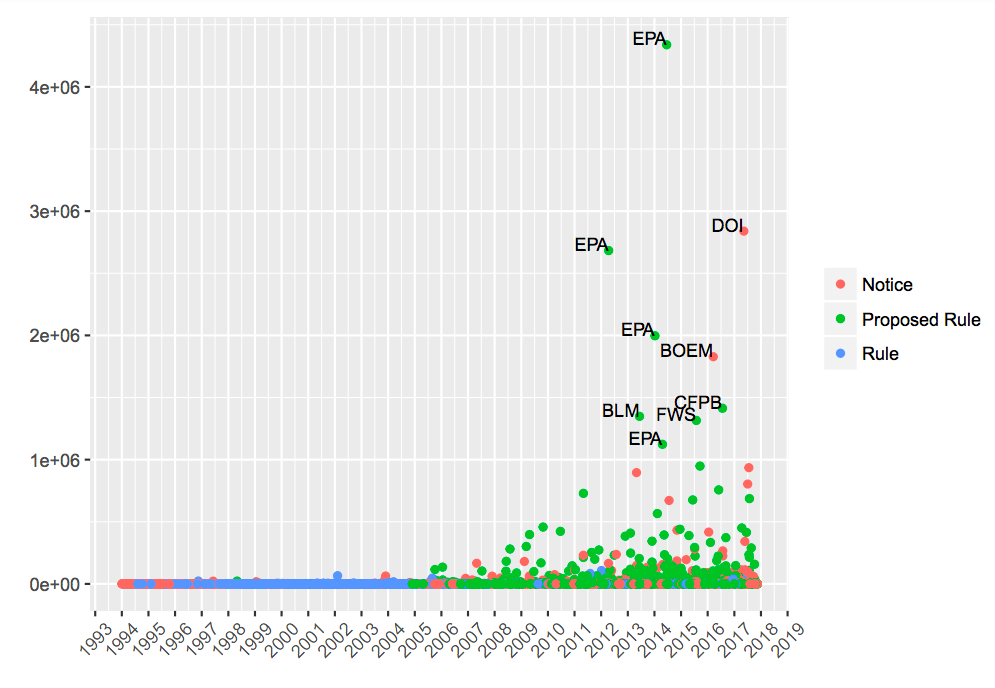
\includegraphics[width= 3in]{number_of_comments}
 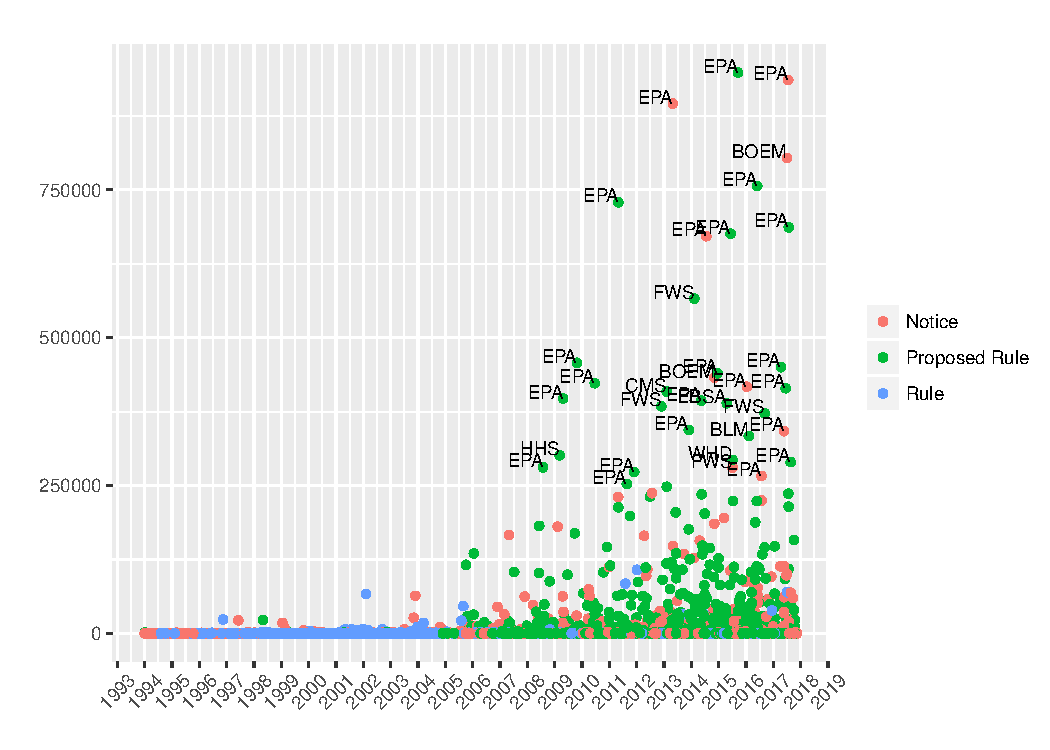
\includegraphics[width = 3in]{comments_under_1m}
\label{fig:comments}
\end{figure}

 

%\section{Outcome Measures}

%\subsection{Goals Achieved}

%The primary outcome is whether the organization achieved its goals. As priors and goals are stated for both the treatment and control rules in the survey that each organization will be asked to fill out, I can assess the difference between treated and untreated rules and whether the number of comments (dosage) is associated with the number of goals achieved. 

%\subsection{Attention and issue framing}
%I will use text analysis to measure three outcomes: First, did the agency respond to the concerns raised in the comments? Comparability requires that the mobilizing organization either submit their own comment (which often more technical than mobilized comments) on both treatment and control rules or submit on neither. As agencies are only required to respond to comments that they deem ``substantive,''  If the mobilizing organization submitted their own comment, response to mobilized comments may be measured as the difference in the length of response in treated and untreated rules. 

%Second, comparing the preamble of the final rule to that of the draft, did the agency use more of the words and phrases matching those in the comments? Rule preambles are non-binding texts that frame the aims of the rule and the response to comments.  If the preambles of treated rules are more likely to include words or phrases from the organizations messaging and mobilized comments, this may indicate agency attention to their demands.\footnote{Recall that  treated and untreated rules both receive at least one comment with the organization's messaging but only treated rules receive a high dosage of it.}

%Third, did the agency adopt language from comments into the text of the policy itself? It is unlikely that language from citizen comments will be sufficiently technical to be adopted into a rule. However, a higher dosage of public comments may make the more technical and legalistic comments of associated organizations more influential.

%Each of these could be dummy variables or continuous measures based on the number of words in the agency response and number of new words and length of new phrases adopted from the comments into the preamble or rule. 
\noindent
Existing data on federal rulemaking are rich, but may not be able to identify whether a campaign influenced a rule or a pending change to a rule inspired the campaign.
For example, we may want to know whether public comments affect compliance with E.O.12898 on addressing Environmental Justice issues. Figure \ref{ejlogitagencies} (Left) shows that %presents results from a logit model, showing the probability that a final rule will include the phrase ``environmental justice'' when the proposed rule did not but comments did. 
the phrase ``environmental justice" being raised in comments is correlated with it being added to a rule. This correlation is especially clear for the EPA, where a comment mentioning ``environmental justice'' is associated with a 10\% increase in the probability that it will be added in the final rule. However, this may occur for many reasons. Figure \ref{ejlogitagencies} (Right) suggests that this change is not correlated with the number of comments received (at least in this simple model). %Furthermore, I have yet to evidence that proposed rules with many comments were more likely to add ``environmental justice'' to the final rule.

Gathering data in real time and testing different strategies may help disentangle how campaigns shape the rulemaking environment from how aspects of a rulemaking may shape campaigns. For example, did campaigns inspire increased attention to environmental justice? Or did agencies' intentions to address E.O.12898 in their final rules inspire commenters to mention it? %If whether environmental justice concerns were raised in comments or not could be experimentally manipulated, this could offer evidence about the causal effect.

\begin{figure}[ht!]
\centering
\caption{Probability that a Final Rule Addresses Environmental Justice when the Proposed Rule Did Not}
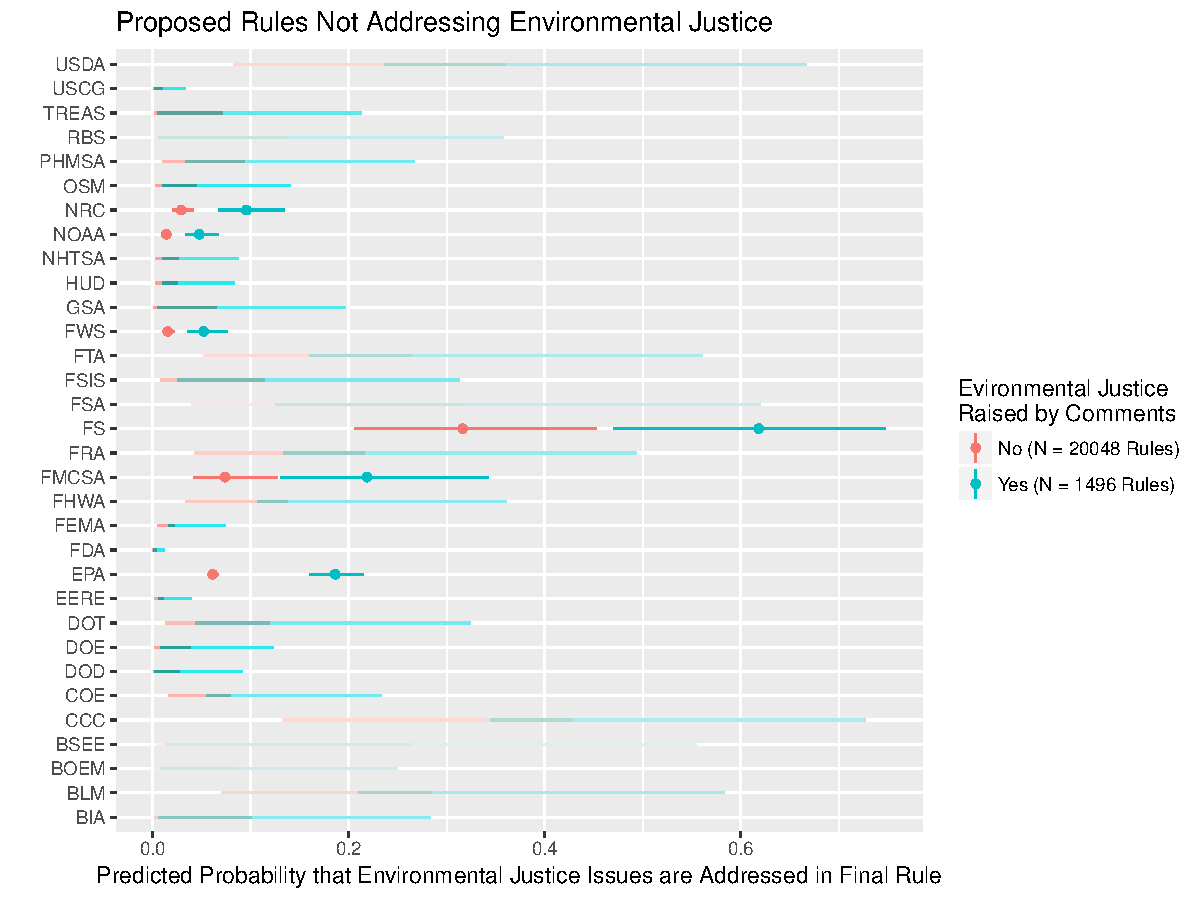
\includegraphics[height = 3in]{ej_prprob_by_agency.pdf}
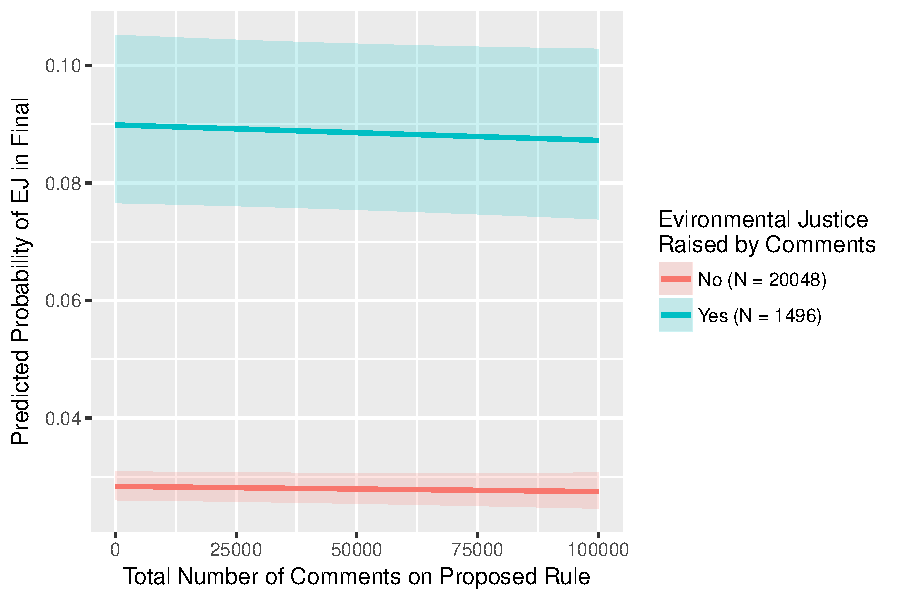
\includegraphics[trim = 0 0 1.65in 0, clip, height = 2in]{ej_prob_env_nprms.pdf}
\label{ejlogitagencies}
\end{figure}


%Having explored the relationship between public comments and policy texts using observational data in the first parts of the dissertation, I turn to a field experiment to identify causal effects.

%The objective of the field experiment is to manipulate public attention on certain proposed rules and measure the agency responses. 

%\section{Case selection: Matching similar proposed rules}

%I am working with activist organizations to identify cases where they will allow me to randomize their advocacy strategy (i.e. whether to run a mass comment campaign) over similar upcoming agency decisions. Ideally, this means that we will identify two upcoming rulemaking processes with similar deadlines and on similar topics managed by the same sub-component of the agency (see examples in the appendix). They will draft objectives and messaging around each. 

%\section{Expert priors: Expected changes with and without large numbers of comments}

%I will survey participating organizations on their expected potential outcomes of the rulemaking process. This includes both the organizations with which I am working and any other organized group that submits comments. 

%I ask for two predicted outcomes: what they predict to occur without public comments and what they hope to achieve by mobilizing public comments (draft survey questions in the appendix).

%\section{Treatment}
%The treatment is the text of public comments sent to the agency. The number comments can be seen as a dosage.\footnote{As the number of citizens mobilized to comment depends on what they are asked to comment on, the dosage is not independent of the treatment.} 

\subsection*{Example research questions}
How do agency staff interpret protests, petitions, and mass commenting? How do the effects of mass mobilization vary across agencies and administrations? How does the processing of public comments (e.g. by staff or contractors) vary across agencies and rules? Are personalized comments interpreted differently than form comments? Do campaigns affect perceptions of public opinion? To what extent do agency staff attribute comments to the organizations that mobilized them? Do they pay more attention to the demands of organizations associated with protests, petitions, and mass-comment campaigns? If public commenting is seen as an expression of intense feelings among a segment of the population, has the increased ease of commenting decreased the weight assigned to each comment?

Does the scale of participation in protests or petitions affect external attention to rulemaking?  To what extent are agency policymakers influenced by media attention and the positions of members of Congress? To what extent does mass mobilization provide ``cover'' for agencies to resist pressure from members of Congress or the White House? 

%\subsection{Potential additional treatment condition: Letters to Congress}

%Additional treatment conditions could be used to test mechanisms directly. For example, if partner organizations are willing and a third similar rule exists, a campaign using the same draft messaging about the proposed rule may ask people to write letters to their member of Congress rather than directly to the agency. 

%This condition would help test the direct causal effect of Congressional attention by inducing letters from members of Congress without public comments. 




%\subsection{Potential additional manipulation: Why mobilize? (science, fairness, voice)}

%Some organizations already do A/B message testing with respect to mobilizing public engagement. If organizations are receptive, I may propose randomizations of messaging based on theories of what influences agency officials. Ideally, this will include activating bureaucrats' reputational concerns as well as threats of political backlash, though credibly manipulating the latter is more difficult. As these messages will be passed through comments, it will be possible to estimate effects on both mobilization and subsequent agency action as a downstream effect (my primary interest).










\section*{Potential mechanisms of influence:}

%It may be impossible to identify the causal mechanisms that lead rule-writers to change policy.
Agency records of internal and external communication about the rulemaking process and interviews with staff who write rules and respond to comments may reveal both direct and indirect effects of campaigns.

% \subsubsection{Why, agencies respond (science, fairness, representation, threat | agency identity)}
% Given prior expectations, assess treatment effects on agency decisions.

\subsection*{Perceptions of public opinion and the `right thing to do'}

The areas of potential change between proposed and final rules are often on such technical questions that it is difficult to know where public opinion lies. One possible mechanism by which comments may influence rule-writers is by subtly reshaping their perceptions of public opinion and the appropriate course of action for a public servant. Studying  the ways in which mass-comment campaigns shape the thinking of and conversations among rule-writers may include interviews and obtaining records of internal correspondence about the rulemaking process through FOIA requests. %I will ask general questions about the particular rulemaking process and the reasoning behind any changes. If subjects mention public comments, I will ask what was compelling about the comments? This may not be an objective measure of these mechanisms, but it may be the closest one can get to knowing how public comments directly affect rule-writers' perceptions. 

\subsection*{External attention and perceived consequences}

Campaigns may also have indirect effects. Instead of directly shaping beliefs about public opinion and the appropriate course of action, they may attract the attention of the media or political principals such as the White House and members of Congress. This attention may then affect beliefs about public opinion and the appropriate course of action. It may also signal potential consequences, such as reversal by Congressional Review, more oversight hearings, or changes in program budgets. %External attention has two forms: general attention, which may increase with increased salience caused by a mass-commenting campaign, and specific attention referencing public comments as a reason for the attention. 

Potential measures of congressional attention include (1) mentions of the rule in congressional testimony (this is rare), (2) communication between members of Congress and agency staff about the proposed rule (slightly more common), and (3) the importance that rule-writers place on congressional attention when interviewed. Measures of attention from the White House include (1) whether the White House Office of Management and Budget requires substantial changes to the rule,  (2) communication between the White House and agency staff regarding the rulemaking process, and (3) the importance rule-writers place on attention from the White House when interviewed. 


\section*{Collaborating to measure campaign effects in real time}

At a minimum, I hope to survey experts who submit comments on behalf of organizations and who organize campaigns targeting agency actions. To allow systematic comparison of expectations with outcomes, I will ask experts and organizers to fill out a short survey before and after the public comment period.

%There are at least two opportunities for random assignment. 
With organizations interested in collaborating more intensively, I hope to develop more innovative approaches to measure the effects of different strategies. For example, we may be able to randomly assign which of an organization's specific goals are addressed in an action alert and thus in mobilized comments. %The email and social media posts mobilizing comments would include messaging only on treated goals. 
I would then measure variation in attention to these goals in the media and among elected officials.
Alternatively, we may randomly assign similar low-salience proposed rules (i.e. rules on which organizations were planning to submit a comment but not planning on sending out an action alert) to treatment and control conditions (e.g. sending out an action alert on the treated rule) and measuring variation in attention and changes between the rules.\footnote{As agencies are required to respond to ``substantive'' comments, their response to the comment in the control condition will be based only on its ``substantiveness.'' In the treatment condition it will be based on substantiveness and volume of public response.} 
%Treated rules will receive a mass commenting campaign, recruiting at least 100, ideally over 1000 citizen comments. 
%Treated rules will receive a mass commenting campaign, recruiting at least 100, ideally over 1000 citizen comments. 

In exchange participating in data collection, I hope to provide analysis of this systematic data on campaign effectiveness. For example, organizations may be interested in how their campaign is generating attention from the media and from elected officials and in the overall distribution of public comments.


\bigskip
\noindent

 


\end{document}

% \subsection{Field experiment 2: Manipulating mechanism (agency, legislators, governor)}











\section{Ethics}
This experiment randomly allocates existing activist resources and attention among policy priorities they see as equivalent, similar to partnering with organizations that mobilize voters. All comments will be the freely expressed opinions of real people. The treatment conditions merely nudge their attention on a particular proposed government action of which they were likely unaware. If treatment effects are observed, public policy may have been affected by the study, but it will not be systematically affected in any particular direction and it would be difficult to argue that this manipulation harms democratic norms.  

For maximum validity, the experiment requires a benign form deception by omission. Citizens and, most importantly, bureaucrats should be unaware that the attention on one rule or issue rather than another is part of a study. It is not fatal to the design if bureaucrats become aware of the study. Many of the mechanisms should still operate, but we may expect lower effects if sentiments expressed in comments are perceived as somehow artificial.

The most significant ethical questions emerge if I end up paying individuals to comment. If research funds are used to pay individuals to comment and they are provided information from a partner organization's campaign, this could be seen as subsidizing the organization's policy efforts. 


\section{Research plan}

\subsection{Pilot}
I will be grateful for any feedback on fielding a pilot. My current plan is to partner with one organization and focus on one pair or trio of proposed rules. I may use undergraduates or MTurkers to increase the number of comments on the treated rule in the pilot study.

\subsection{Study}
Starting in Summer 2018, I will begin recruiting organizations that mobilize mass commenting to participate in my study. An organization may opt to participate in the survey only or in surveys and field experiments. %The survey will 

\newpage

\section*{Appendix 1: Example pair of draft regulations from the Fish and Wildlife Service's Endangered Species Program}

A. 

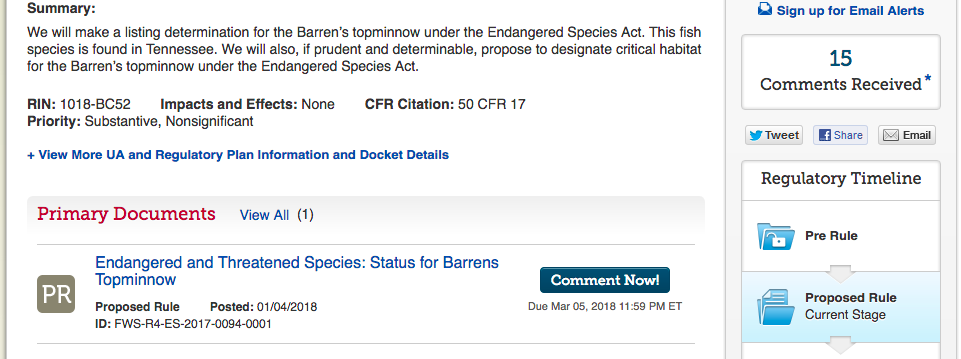
\includegraphics[width = \textwidth]{topminnow.png}

\noindent B. 

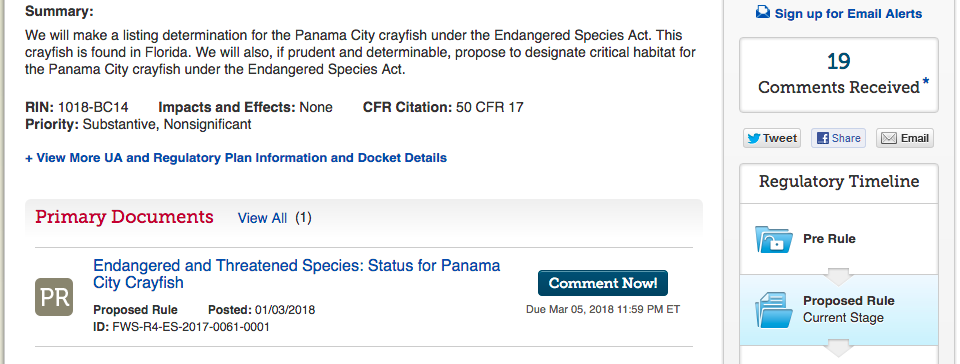
\includegraphics[width = \textwidth]{crayfish.png}

\newpage

\section*{Appendix 2: Example pair of draft regulations from the EPA Office of Air and Radiation}

A. 

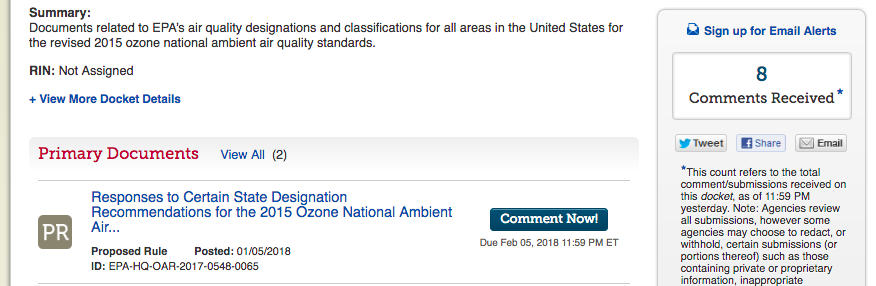
\includegraphics[width = \textwidth]{ozone.png}

\noindent B. 

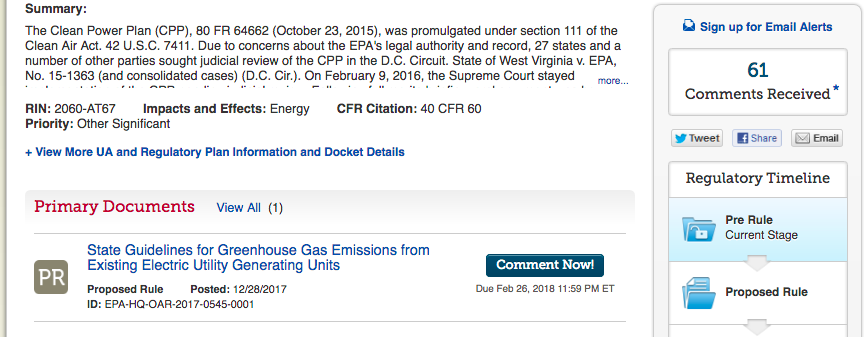
\includegraphics[width = \textwidth]{CPP.png}

\newpage
\section*{Appendix 3: Survey}

This survey aims to track the effectiveness of participation in notice-and-comment rulemaking. In exchange for your participation, you will receive an annual report analyzing your success as well as aggregate trends. Please answer honestly to the best of your knowledge. \textit{Your specific answers and report are confidential}. The more detailed information you are able to provide, the more informative the results will be.

\doublespace
\bigskip
\tiny

1. \textbf{Who is likely to participate in this notice-and-comment process?}

1.1 Do you have formal coalition partners? If so, please list them:

\fbox{\color{gray} ..............................................}


1.2 Who else is likely to comment \textit{in alignment} with your goals:

\fbox{\color{gray} ..............................................}

1.3 Who is likely to comment \textit{in opposition} to your goals:

\fbox{\color{gray} ..............................................}

Other likely commenters (neither aligned nor opposing): 

\fbox{\color{gray} ..............................................}

About how many total comments do you estimate will be received:

\fbox{\color{gray} ..............................................}

If your coalition is mobilizing citizen comments, how many do you anticipate mobilizing: 

\fbox{\color{gray} ..............................................}

\bigskip


2. \textbf{Why are you participating in this notice and comment process?}


In general: 

\fbox{\color{gray} ..............................................}

2.1 Briefly describe any procedural aims or complaints:

 \fbox{\color{gray} ..............................................}

2.2 Briefly describe any substantive goals:

\fbox{\color{gray} ..............................................}

\begin{tabular}{l c c c}
& Probability & Desired & Undesired \\
\hline\\
Withdrawal & \fbox{\color{gray} XX}\% & \fbox{\checkmark} & \fbox{\checkmark}  \\
Delay & \fbox{\color{gray} XX}\% & \fbox{\checkmark}& \fbox{\checkmark}  \\
Major revision & \fbox{\color{gray} XX}\% & \fbox{\checkmark} & \fbox{\checkmark} \\
\fbox{\color{gray} Other}  & \fbox{\color{gray} XX}\% & \fbox{\checkmark}  & \fbox{\checkmark}  \\
\ovalbox{\color{blue} Add potential outcome}\\
\end{tabular}

\bigskip
\singlespace

2.3 Please describe any specific potential revisions, including specific hopes, fears, and expectations, ideally specific bits of draft text that may change. Please check changes targeted by your coalition. For example any of the hoped policy changes that you suggest and any feared policy changes you argue against.

\bigskip

\doublespace
\begin{tabular}{c c c c c | c}
\small
\noindent
Targeted & Current & Potential & \multicolumn{2}{c}{\underline{Probability of change (your guess)}} & Was this change made?\\
this change?& text& text & Without comments & With comments & [AFTER FINAL PUBLISHED]\\
\hline\\
\textbf{Hopes:} &\\
(1) \fbox{\checkmark}  & \fbox{\color{gray} Old text} & \fbox{\color{gray} New text} & \fbox{\color{gray} XX}\% & \fbox{\color{gray} XX}\% & Yes \fbox{\checkmark} No \fbox{\checkmark} Partial \fbox{\checkmark}\\
 \\
\ovalbox{\color{blue} Add hope}\\
\hline\\
\textbf{Fears:} &\\
(1) \fbox{\checkmark}  & \fbox{\color{gray} Old text} & \fbox{\color{gray} New text} & \fbox{\color{gray} XX}\% & \fbox{\color{gray} XX}\% & Yes \fbox{\checkmark} No \fbox{\checkmark} Partial \fbox{\checkmark}\\
 \\ \ovalbox{\color{blue} Add fear}\\
\hline\\
\textbf{Other expectations:} &\\
(1) \fbox{\checkmark}  & \fbox{\color{gray} Old text} & \fbox{\color{gray} New text} & \fbox{\color{gray} XX}\% & \fbox{\color{gray} XX}\% & Yes \fbox{\checkmark} No \fbox{\checkmark} Partial \fbox{\checkmark}\\
 \\
\ovalbox{\color{blue} Add expectation}\\
\end{tabular}






\newpage
% bib style: I recommend a permanent pathway to this file!
\bibliographystyle{apsr.bst} 
% bib file: I recommend a permanent pathway to this file!
\bibliography{Mendeley.bib}
\end{document}

catagories of outcomes 
- by theory 

meaningful 
- less meaningful is response
- most is policy change 

panel of experts 

if there are not comments 

double barrel treatment 
- the effect could be due to the campaing or comments 



what can you measure?
- what does theory suggest we should see 



survey exp?
- hard to get people?
- 


policy chnage 
1 - as experts wanted
2 - in one direction or the other 
3 - more similar words to one coalition 


what is actually happening?
- mechanisms 
- how it works
- foia congress
- foia communications 

- interview them - 


elite interviews
- tell me about this rule
- tell me about this change
- what was so compelling about the comments 

effect of campign 

anything above nothing 



READ 
- POWER 
- MEDIATION AND MECHANISMS - how difficult it is to learn about mechanisms


PROSPECTUS: 

Dear Last Week Tonight team,
I am a doctoral candidate in political science. I am designing a series of experiments to test the functioning of American democracy and write to ask if you would like to collaborate. 

These experiments aim to test the effects of mass citizen engagement in policy areas like flood zone maps, internet regulations, and banking regulations that often seem too complex or technocratic—i.e. your specialty. Experiments may allow us to quantify and causally identify the impact of you and your viewers.

Specifically, we hope to match similar pending agency actions that are not receiving a lot of attention and randomize a ‘treatment’ that increases participation in the public comment process. With randomized treatment we can observe the effects off mass engagement on outcomes like agencies’ official response to comments, changes in rule text, and communication between members of Congress and agencies, which I have been collecting through FOIA requests.

I am working with Professor Susan Yackee who has conducted the most cited work on the question of who gets heard in the public comment process, finding that it is mostly businesses, but that opposing comments may blunt business influence. Scholars have yet, however, to examine whether mass commenting like the kind you generated on the open Internet rules matters, and if so, how.

I am very open to working on topics or formats of your choosing but am also happy to suggest agency actions worthy of attention. Our study only requires some kind of randomization between treatment and control conditions for similar policies. This could be as simple as tweeting about one policy and not the other. Or perhaps, if two similar environmental regulations both illustrate your point, you could flip a coin to choose which one to highlight, and let me know the road not taken. 

After we complete this analysis, I imagine interesting publicity opportunities regardless of the results. Where we find effects, it may inspire more of your viewers to engage. Where we do not, it raises interesting questions about  these mechanisms of democracy.

Please let me know if anyone on your team is interested in discussing this further. 

Best,
Devin 